%
% BUS 238: Introduction to Entrepreneurship and Innovation
%
% Author: Jeffrey Leung
%

\documentclass[10pt, oneside, letterpaper, titlepage]{article}

\usepackage[ampersand]{easylist}
	\ListProperties(
		Progressive*=5ex,
		Space=5pt,
		Space*=5pt,
		Style1*=\textbullet\ \ ,
		Style2*=\begin{normalfont}\begin{bfseries}\textendash\end{bfseries}\end{normalfont} \ \ ,
		Style3*=\textasteriskcentered\ \ ,
		Style4*=\begin{normalfont}\begin{bfseries}\textperiodcentered\end{bfseries}\end{normalfont}\ \ ,
		Style5*=\textbullet\ \ ,
		Style6*=\begin{normalfont}\begin{bfseries}\textendash\end{bfseries}\end{normalfont}\ \ ,
		Style7*=\textasteriskcentered\ \ ,
		Style8*=\begin{normalfont}\begin{bfseries}\textperiodcentered\end{bfseries}\end{normalfont}\ \ ,
		Hide1=1,
		Hide2=2,
		Hide3=3,
		Hide4=4,
		Hide5=5,
		Hide6=6,
		Hide7=7,
		Hide8=8 )
\usepackage{geometry}
	\geometry{margin=1.2in}
\usepackage{graphicx}
	\graphicspath{ {img/} }
\usepackage[colorlinks=true, linkcolor=blue]{hyperref}
\usepackage{lmodern} % Allows the use of symbols in font size 10; http://ctan.org/pkg/lm
\usepackage{pdfpages}
\usepackage{textcomp} % Allows the use of \textbullet with the font
\usepackage{verbatim}

\renewcommand{\arraystretch}{1.2}
\renewcommand{\familydefault}{\sfdefault}

\title{BUS 238: Introduction to Entrepreneurship and Innovation \\\medskip \Large A Course Overview}
\author{Jeffrey Leung \\ Simon Fraser University}
\date{Fall 2017}

\begin{document}

	\maketitle
	\tableofcontents
	\clearpage

	%
% CMPT 213: Object Oriented Design in Java - A Course Overview
% Section: Introduction
%
% Author: Jeffrey Leung
%

\section{Introduction}
	\label{sec:introduction}
\begin{easylist}

& Standards:
	&& Make fields private when possible

& Commenting:
	&& Comment purpose of a class
	&& Name fields/methods/parameters so comments are unnecessary

& When possible, convert strings to non-string types internally for consistency

& \textbf{Clean code:} Code which is correct, easy to read/maintain, and conforms to a standard

& Software design:
	&& 4 steps:
		&&& Requirements
		&&& Design and implementation
		&&& Verification
		&&& Evolution
	&& Designing involves identifying classes, responsibilities, and relationships to create a diagram
	&& Implementation process options:
		&&& \textbf{Skeleton code:} Beginning minimal parts/features of a system
		&&& \textbf{Component-wise:} Creating components one at a time
	&& Methods of integrating code from multiple people:
		&&& \textbf{Continual integration:} Gradual system growth by constantly integrating changes
		&&& \textbf{Big Bang integration:} Building all parts separately without integrating until the end

& \textbf{Feature envy:} Characteristic of a class which relies heavily on another class
& Warning sign: Characteristic of a method which operates more strongly on another object than its own
& \textbf{Deprecation:} State where a public interface is no longer supported or recommended, and is slated to be removed in the future


& \textbf{try-catch:} Structure which watches for an exception and handles it
	&& Only one exception can be live at a given time
	&& \textbf{finally clause:} Optional clause after catch clauses which is executed regardless of the result
		&&& If exception is thrown, the finally clause is executed immediately afterwards
	&& \textbf{try-with-resources:} Block which cleans up a resource when a try block exits

& Exception: Issue which may be fixable and is not out of the software's control
	&& \textbf{Checked exception:} Exception which must be caught or listed in a throws clause
	&& \textbf{Unchecked exception:} Exception which will automatically propagate and does not require catching
		&&& E.g. RuntimeException
		&&& Preferred as it does not require modification of methods between try/catch, which decouples code

\end{easylist}
\clearpage

	%
% BUS 238: Introduction to Entrepreneurship and Innovation
% Section: Innovation
%
% Author: Jeffrey Leung
%

\section{Innovation}
	\label{sec:innovation}
\begin{easylist}

& \textbf{Innovation:} Improving or changing an idea or item to meet a need
	&& Involves matching technoogy to a market application
	&& Not the invention of something new
	&& Iterative to improve competition and to solve problems
	&& Involves value-add and newness
	&& Aims for seamless adoption of influential change

& Types of innovation:
	&& \textbf{Product/Service innovation:} Changing an offering to customers
	&& \textbf{Process innovation:} Changing the creation, composition, and/or maintenance of a product or service
		&&& Often in the interest of efficiency and cost
	&& \textbf{Marketing innovation (positioning):} Changing how an offering is portrayed in communications
	&& \textbf{Platform innovation:} Changing the foundation on which other businesses or processes operate
	&& \textbf{Business model innovation:} Changing the model of thought of the priorities and operations
		&&& E.g. RyanAir is a airline which provides low quality services at low costs
		&&& E.g. Netflix is a media streaming service which moved subscription services and distribution to online
	&& \textbf{Social innovation:} Creating solutions to social and/or environmental issues/deficits
		&&& Often target market weaknesses or address market failures
	&& \textbf{Sustainable innovation:}
		&&& Long-term maintenance of a concept or solution while creating the least environmental impact and utilizing all the possible resources

& Speed and impact of innovation:
	&& Incremental (e.g. parking services)
	&& Substantial (e.g. remote engine diagnostics)
	&& Radical (e.g. hybrid engine technology)

\end{easylist}
\clearpage

	%
% BUS 238: Introduction to Entrepreneurship and Innovation
% Section: Entrepreneurship
%
% Author: Jeffrey Leung
%

\section{Entrepreneurship}
	\label{sec:entrepreneurship}
\begin{easylist}

& \emph{Entrepreneurship:} Creation of purposeful and focused change in an enterprise's economic/social potential
	&& Often without regard to resources currently controlled
	&& Innovating a new product, creating a new business model, improving a product

& \emph{Opportunity:}

& \emph{Pursuit:} Following the realization of an opportunity, often with focus and urgency

& \emph{Beyond resources controlled:} Need to identify and access external resources to support the realization of opportunity

& Steve Blank: Entrepreneur and originator of the Lean method
	&& \href{https://steveblank.com}{Website}

& \emph{Intrapreneurship:} Being an entrepreneur within a company

& To create impact:
	&& Think like a movement to create social change
	&& Create a container for content delievered to consumers
	&& Be ready to engage with allies, adversaries, and strangers
	&& Leverage your economic power and reduce reliance on others
	&& Advocate for causes in an empathetic way
	&& Understand who should be in your circle

\end{easylist}
\clearpage

	%
% BUS 238: Introduction to Entrepreneurship and Innovation
% Section: Problems
%
% Author: Jeffrey Leung
%

\section{Problems}
	\label{sec:problems}
\subsection{Root Cause Analysis}
	\label{subsec:root-cause-analysis}
\begin{easylist}

& Steps:
	&& Identify the problem and key indicator/symptom
	&& Iteratively identify any linked causes
	&& Identify the furthest root causes

& When creating an RCA:
	&& Don't leap to conclusions
	&& Focus on direct causations
	&& Consider context of each causation
	&& Create many branches

& \emph{Insight:} Understanding the underlying nature of a concept
	&& User insight:
		&&& Revelation about an aspect of users
		&&& Realization of new opportunities
	&& Methods of gaining insight:
		&&& \emph{Observation:} Perception of behaviour without interfering interaction
			&&&& Should be objective about behaviour and not include emotions or make inferrances
			&&&& Using observations, find insights
			&&&& \emph{POEMS framework:} When observing, pay attention to People, Objects, Environments, Messages, and Services
				&&&&& People: Who is present/involved?
				&&&&& Objects: What is involved? (e.g. equipment, materials, product, infrastructure)
				&&&&& Environments: Uniqueness in and characteristics of the environment (e.g. noise, temperature, crowdedness, privacy, security, atmosphere)
				&&&&& Messages: Information conveyed by/from people (e.g. other people in the vicinity, environment, advertising, promotions)
				&&&&& Services: Services offered and results
			&&&& Pay attention to:
				&&&&& Disjunctures and inconsistencies with previous understandings/observations
				&&&&& Revelatory incident which requires explanation and contextualization
				&&&&& Personal interpretations and differences between what is said and what is done
				&&&&& Cultural contextual issues
				&&&&& Metaphorical and symbolical experiences relating to a larger concept

\end{easylist}
\subsection{Empathy Mapping}
	\label{subsec:problems:empathy-mapping}
\begin{easylist}

& Discuss with people to understand the problem better

\end{easylist}
\clearpage

	%
% BUS 238: Introduction to Entrepreneurship and Innovation
% Section: Interviewing
%
% Author: Jeffrey Leung
%

\section{Interviewing}
	\label{sec:interviewing}
\begin{easylist}

& Recommendations:
  && Listen actively
	&& Ask for history or context
	&& Ask follow-up questions to encourage deeper discussion
	&& Encourage them to tell stories

& Refrain from:
	&& Asking leading questions
	&& Asking yes/no questions
	&& Asking obvious questions
	&& Making predictions or assumptions

\end{easylist}
\clearpage

	%
% BUS 238: Introduction to Entrepreneurship and Innovation
% Section: Creativity
%
% Author: Jeffrey Leung
%

\section{Creativity}
	\label{sec:creativity}
\begin{easylist}

& \emph{Creativity:} Solution which is both relevant to the problem and novel
	&& Irrelevant to artistry
	&& Can be practiced and improved

& \emph{Brainwriting:} Individual idea generation
& \emph{Brainstorming:} Social idea generation
	&& Build off of others' ideas
	&& Don't criticize ideas

& When being creative:
	&& Do not self-filter
	&& Prioritize quantity over quality
	&& Create wildly unrealistic ideas

& SCAMPER framework:
	&& \textbf{S}ubstitute one concept for another
		&&& E.g. Replace meat with tofu
	&& \textbf{C}ombining multiple concepts
		&&& E.g. Adding two cuisines
	&& \textbf{A}dapting concepts for another environment
		&&& E.g. Chinese food in the US
	&& \textbf{M}odify existing concepts
		&&& E.g. Use cereal to create cereal bars
	&& \textbf{P}ut a concept to another use
		&&& E.g. Using food as art
	&& \textbf{E}liminate a concept from its context
		&&& E.g. Remove meat from burgers
	&& \textbf{R}everse
		&&& E.g. Wrap the dough of a pizza around the toppings to create a calzone

\end{easylist}
\clearpage

	%
% BUS 338: Foundations of Innovation - A Course Overview
% Section: Marketing
%
% Author: Jeffrey Leung
%

\section{Marketing}
	\label{sec:marketing}
\subsection{Markets and Segments}
	\label{subsec:markets-and-segments}
\begin{easylist}

& \textbf{Marketing:} Strategy and process of identifying, targeting, engaging, and acquiring customers

& \textbf{Market:} Set of consumers who have similar perceptions and preferences, have specific needs and desires fulfilled by a set of products or services, and who reference each other when making a buying decision
	&& Types of market:
		&&& \textbf{Clone market:} Consumers who will buy into a copy of an existing business model
		&&& \textbf{Existing market:} Consumers who will purchase a higher-end product which is faster, more efficient, etc.
		&&& \textbf{Cheaper segmented existing market:} Consumers who will purchase a lower-end product
		&&& \textbf{Niche segmented existing market:} Consumers who will purchase a product with distinct marketing/branding
		&&& \textbf{New market:} Consumers in a unique new class grouped by a new factor
	&& Characteristics of a market:
		&&& Customers: Needs/pain points, adoption details
		&&& Nature of the market: Size, entry cost, competitive barriers
		&&& Sales margins
		&&& Time to profitability

& Learn about markets by researching:
	&& Government statistics
	&& Industry sources and reports
	&& Companies currently in the industry
	&& People you know from the industry
	&& Interviews/surveys/focus groups with current customers, lead users, field experts

& \textbf{Market segment:} Group of consumers who have common needs and desires who can be targeted by their common perceptions, preferences, and drives, and can reference each other in the buying decision process
	&& Possible segmentation factors: Product usage, demographics, psychographics (personality, values, interests, lifestyle), geography
	&& Segment based on the customers' perceived value, buying process, and behaviours
	&& Do not segment based on demographics, unknown internal behaviours, competitors' segmentation
	&& Process of segmentation: Document market sizing details, determine scoring criteria, determine segment attractiveness, choose initial target segment, select market targets
	&& Characteristics of a segment: End user, needs, urgency of needs, benefit, lead customer, willingness to change/adapt, cost of entry, frequency of buying, size of market, competitive barriers, type of market (clone, resegmented, existing, new)
	&& \textbf{Beachhead segment:} Market segment which is the initial domination target by a product
		&&& Should be small enough to dominate, large enough to have an impact, and be strategically aligned with the product's strengths and weaknesses

& \textbf{Sales-driven marketing:} Positioning of a product to attract any buyer regardless of their characteristic
	&& Initially more attractive than market-driven because of the immediate interest
	&& Eventually will fail and lead to low sales
& \textbf{Market-driven marketing:} Positioning of a product to attract only buyers with specific characteristics
	&& More effective than market-driven because of the ability to dominate a market segment and create cohesive references between buyers

\end{easylist}
\subsection{Positioning Statements and Value propositions}
	\label{subsec:positioning-value}
\begin{easylist}

& \textbf{Positioning:} Portrayal of a product in the mind of the consumer by the company, through marketing in contrast to the competitors
	&& Focuses on customer needs/pains, value of the product, and differentiation from competing products
	&& One positioning statement per target market segment, and one positioning statement for the entire market
	&& Composition of a positioning statement:
		&&& For \textit{target customers} \\
		Who need \textit{compelling reason to buy} \\
		Our product is a \textit{new product category} \\
		That provides \textit{key problem-solving capability; addresses the reason to buy}. \\
		Unlike \textit{competitors' alternative products}, \\
		Our product \textit{key product features and differentiation}. \\
		We also provide \textit{other parts of the product}.

& Types of buyers:
	&& Each target market has a unique set of buyers
	&& \textbf{User buyers}: Group of people who will be using the product or managing the users (i.e. end-users)
	&& \textbf{Technical buyers}: Group of people who do not choose the product, but must approve the purchase (e.g. finance department, regulators, parents)
	&& \textbf{Economic buyers}: Group of people who have the ability to pay for the product (e.g. CEO, CFO, management team, parents)

& \textbf{Value proposition:} Statement about the product's benefits to a specific group of buyers
	&& Varies per audience (one per buyer type per market, and one for each other player in the market - e.g. influencers)
	&& Composition of a value proposition:
		&&& We believe that \textit{target customers} \\
		Should be able to \textit{ability to address need} \\
		By \textit{specific measurement or KPI \#, \$, \%} \\
		Through the ability to \textit{key problem-solving capability; addresses the reason to buy} \\
		As a result of \textit{key product features and differentiation} \\
		For an investment of approximately \textit{\$ estimate}.
	&& Examples:
		&&& \textit{User buyer:} We believe that transfusion nurses \\
		Should be able to reduce transfusion labour \\
		By 75\% \\
		Through the ability to eliminate the 2\textsuperscript{nd} nurse checker and simplify the transfusion process \\
		As a result of implementing barcode cross-checking at the bedside \\
		For an investment of approximately \$200,000.
		&&& \textit{User manager buyer:} We believe that hospital blood bank managers \\
		Should be able to reduce blood bank labour \\
		By 30\% while maintaining existing service levels \\
		Through the ability to allocate blood just-in-time rather than in advance \\
		As a result of implementing on-demand blood issuing \\
		For an investment of approximately \$200,000.
		&&& \textit{Economic buyer:} We believe that hospital CFOs \\
		Should be able to reduce the overall cost of blood transfusions \\
		By 10\% \\
		Through the ability to eliminate wasted blood products and reduce blood inventory levels \\
		As a result of introducing blood tracking and on-demand blood issuing \\
		For an investment of approximately \$200,000.

\end{easylist}
\subsection{Market Adoption Cycle}
	\label{subsec:market-adoption-cycle}
\begin{easylist}

& \textbf{Market Adoption Cycle:} Segmentation of potential buyers by their willingness to adopt an innovation
	&& See figure~\ref{fig:market-adoption-cycle}

\begin{figure}[!htb]
	\centering
	\caption{Market Adoption Cycle}
	\label{fig:market-adoption-cycle}
	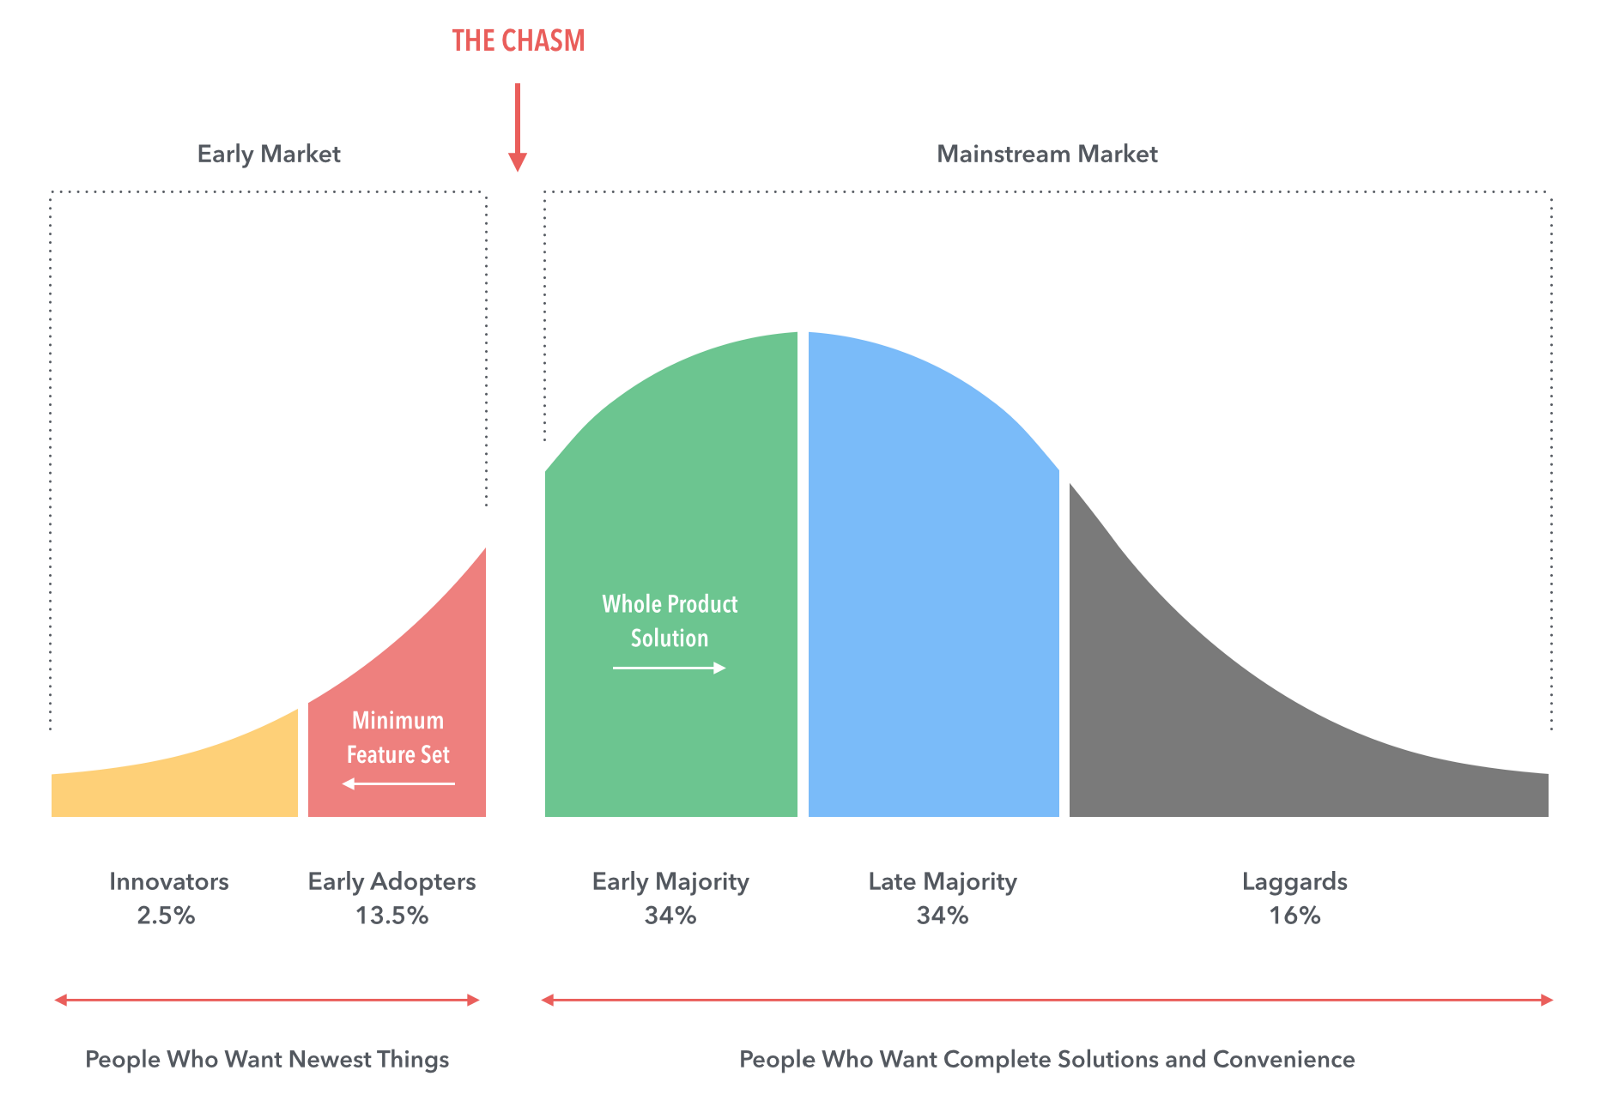
\includegraphics[width=0.7\textwidth]{market-adoption-cycle}
\end{figure}

& \textbf{Innovators:} Enthusiast buyers who actively seek out new innovations
	&& Innovation for the sake of innovation
	&& Desire to be early buyers
	&& Forgiving of and willing to work to resolve problems
& \textbf{Early adopters:} Visionary buyers who use intuition to choose innovations for their own needs
	&& Willing to buy in early
	&& Expectations of significant change from existing solutions
	&& Not price-sensitive
& \textbf{Early majority:} Pragmatist buyers who buy technologies which are proven by market leaders
	&& Larger population
	&& Highly practical
	&& Expectations of incremental change from existing solutions
	&& Require a complete solution
& \textbf{Late majority:} Comfortable buyers who only buy products which are easy to use and safe against decay over time
	&& Larger population
	&& Need support
	&& Need the market to already be dominated by the product
& \textbf{Laggards:} Reluctant buyers who dislike new innovations and will only buy technology which is absolutely necessary

& Characteristics of adopting an innovation:
	&& Relative advantage over existing offerings
	&& Visible and easily understandable value and use
	&& Ease of use when moving from an existing offering
	&& Compatibility with pre-existing conditions and environmental factors

\end{easylist}
\subsection{Pitching}
	\label{subsec:pitching}
\begin{easylist}

& Structure of a pitch:
	\begin{enumerate}
		\item Introductions
		\item The problem and those who experience it
		\item Impact of the problem
		\item Current situation and solutions
		\item Our solution and its desired outcome
		\item Solution's benefits (not features/details)
		\item Competitors
		\item Unique positioning/differentiator and how it benefits the user
		\item Where we have an advantage
		\item Make an ask
	\end{enumerate}

\end{easylist}
\clearpage
	%
% BUS 238: Introduction to Entrepreneurship and Innovation
% Section: Teamwork
%
% Author: Jeffrey Leung
%

\section{Teamwork}
	\label{sec:teamwork}
\begin{easylist}

& Interdisciplinary teams:
	&& Make unique contributions
	&& Reduce errors or tunnel vision
	&& Have greater flexibility
	&& Are more united
	&& Learn more broadly
	&& Reduce communication gaps between industries
	&& Allow people to focus on their strength
	&& Require patience and listening
	&& Are not easy to align goals and direction
	&& Are not put into practice often

\end{easylist}
\clearpage

	%
% BUS 238: Introduction to Entrepreneurship and Innovation
% Section: Business Models
%
% Author: Jeffrey Leung
%

\section{Business Models}
	\label{sec:business-models}
\subsection{Overview}
	\label{subsec:business-models:overview}
\begin{easylist}

& \textbf{Business model:} Description of the organization and finances of a business
& \textbf{Business strategy:} Description of how a business succeeds in relation to competitors
& \textbf{Business plan:} Document describing the business strategy for a particular goal

& \textbf{Vision:} End purpose of your company's existence and the ultimate goals it works to achieve

\end{easylist}
\subsection{Types of Business Models}
	\label{subsec:business-models:types-of-business-models}
\begin{easylist}

& \textbf{Subscription:} Recurring fee to obtain access to a service
& \textbf{Freemium:} A basic offering of a service for free and an improved offering of the service for a price
& \textbf{Fractionalization:} Selling the partial use or ownership of an object or service
& \textbf{Product to service:} Selling a service provided by a product rather than the product itself
& \textbf{Crowdsourcing:} Contribution of content or finances from a large group of people who receive other people's content or are able to see the product succeed
& \textbf{Razor-blade:} Selling a high-margin product below cost to encourage more sales of the low-margin product
	&& E.g. Razors are sold at a low cost to encourage the sale of razor blades
	&& E.g. Printers are sold at a low cost to encourage the sale of ink cartridges
& \textbf{Reverse razor-blade:} Selling a low-margin product below cost to encourage more sales of the high-margin product
	&& E.g. Amazon Kindles are sold at an affordable price to encourage sales of digital e-books
& \textbf{Customization:} Allowing a customer to modify and choose aspects of a product or service
& \textbf{Low touch:} Decreasing service to lower prices
	&& E.g. Self-assembly furniture

\end{easylist}
\subsection{Business Model Canvas}
	\label{subsec:business-models:business-model-canvas}
\begin{easylist}

& Business model canvas: \hyperref[sec:appendices]{see Appendices}

& Customer segments: Small niche type of consumers who is your perfect market and who you create value for
& Value proposition: The value uniquely offered to the customers
& Channels: How customers access the offered value
& Customer relationships: Building rapport with customers
& Revenue streams: Where revenue comes from
	&& Personal rewards
& Key resources: Items, products, people, or concepts critical to your success
& Key activities: Actions undertaken to create value and reach success
& Key partners: Individuals and organizations to work with
	&& Benefits and risks
& Cost structure: What and how consumers pay for the service

\end{easylist}
\clearpage

	%
% BUS 338: Foundations of Innovation - A Course Overview
% Section: Appendices
%
% Author: Jeffrey Leung
%

\section{Appendix A: Business Model Canvas}
	\label{sec:appendix-a}

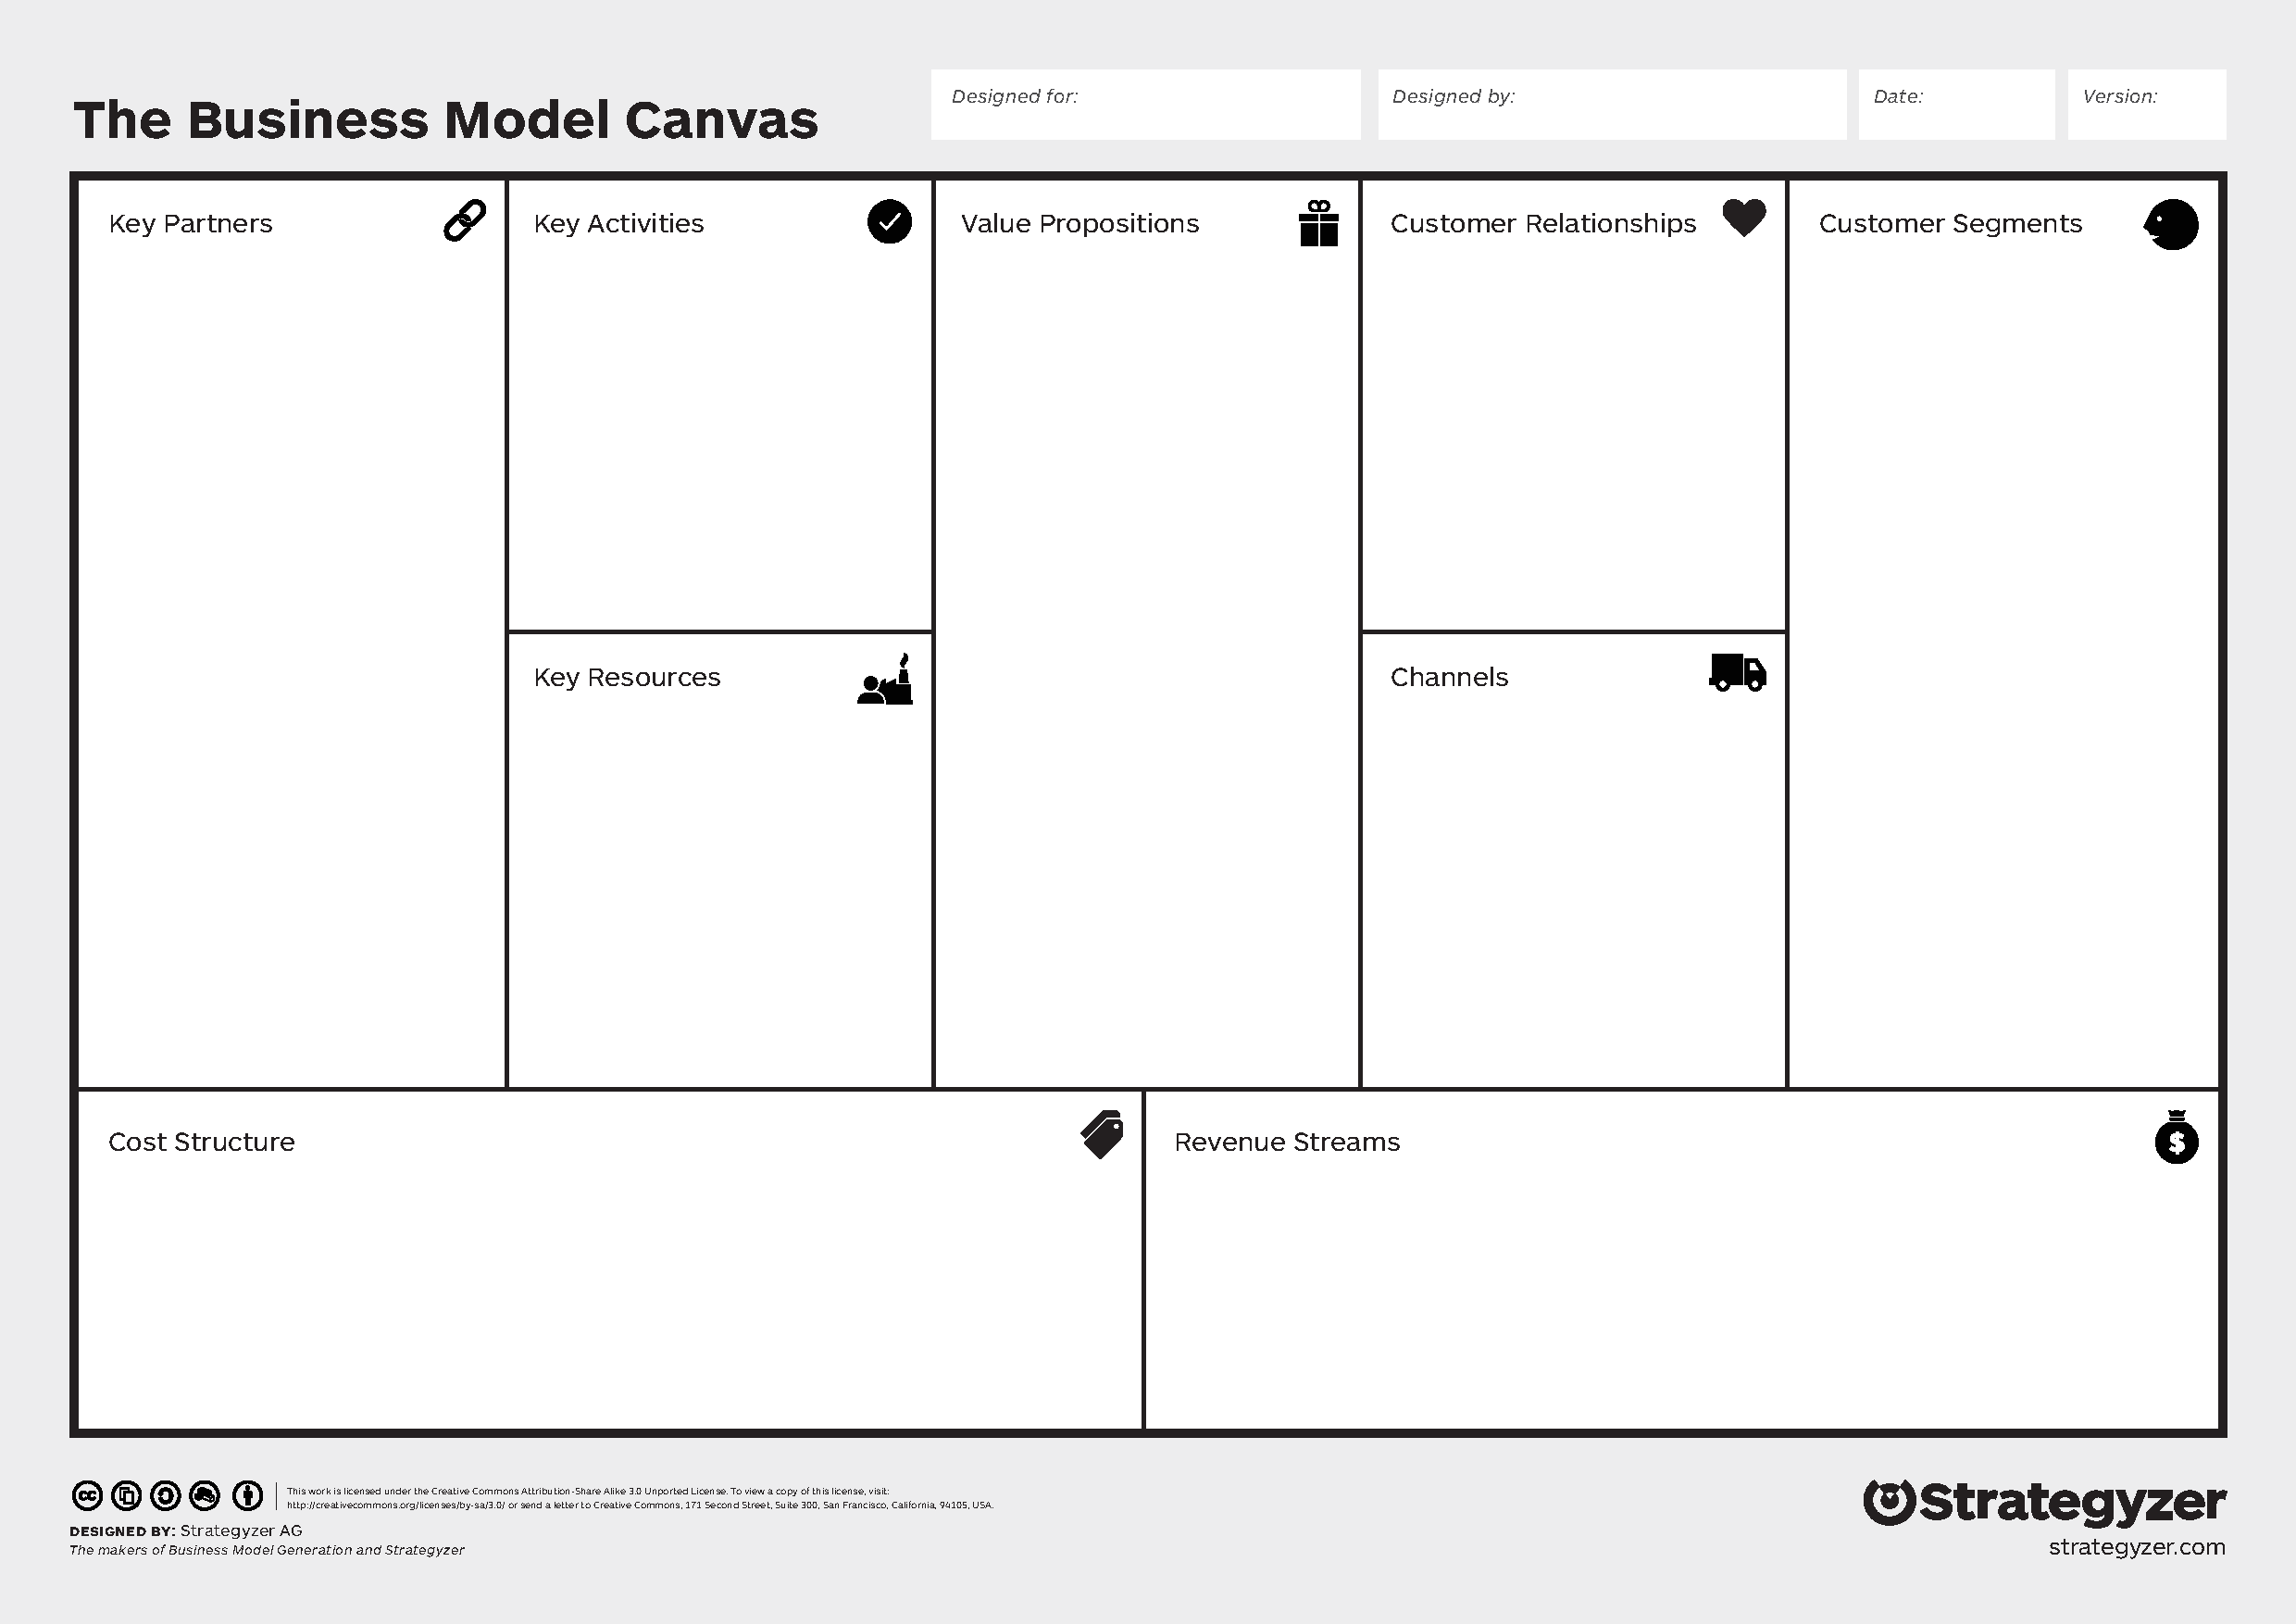
\includepdf[pages={-},landscape=true]{business-model-canvas.pdf}

\clearpage

\end{document}
